\documentclass{article}

\usepackage{stix2}
\usepackage{amsmath}\usepackage{amssymb}\usepackage{amsfonts}
\DeclareMathOperator{\s}{\mathscr{s}}

\usepackage[a4paper]{geometry}
\usepackage{siunitx}
\usepackage{circuitikz}\usepackage{pgfplots}

\usetikzlibrary{pgfplots.smithchart}

\title{ECE218A --- Lab 01A}
\author{George Higgins Hutchinson \& Shouyan Li}

\begin{document}
\maketitle

\section{Introduction}
In this lab assignment, we used a Keysight <Insert actual model name here> VNA to measure several important properties for passive devices.

\section{Methods}

\section{Results}
\begin{figure}
  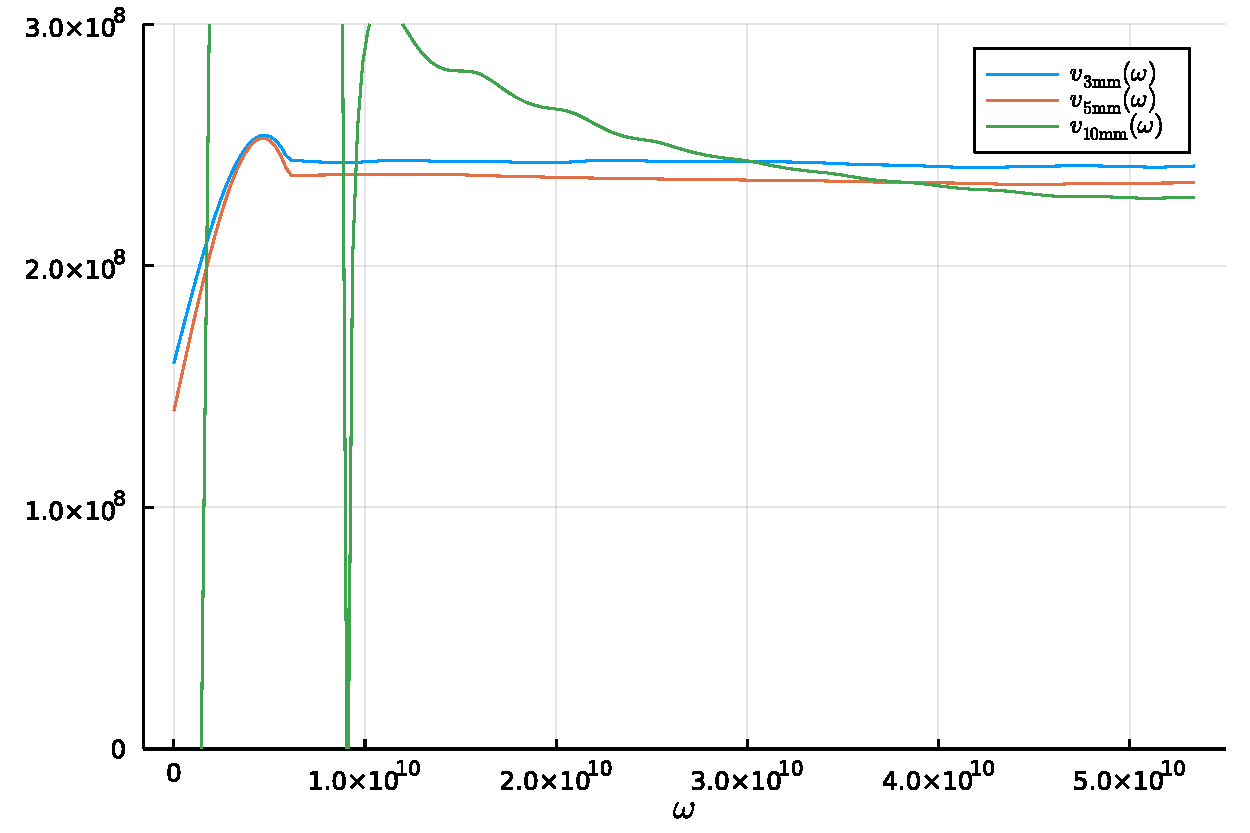
\includegraphics[width=0.8\textwidth]{figures/build/phase_vel.pdf}
  \caption{Effective phase velocity, measured for excitations at angular frequency $\omega$.}
\end{figure}
\end{document}

